%%%%%%%%%%%%%%%%%%%%%%%%%%%%%%%%%%%%%%%%%
%% Appendix section
% Set-up the section.
\newpage
\appendix
\setcounter{table}{0}
\renewcommand{\thetable}{A\arabic{table}}
\setcounter{figure}{0}
\renewcommand{\thefigure}{A\arabic{figure}}

% Start appendix
\section{Appendix}
\label{appendix}
This project used data which are fully public, and computational tools which are fully open-source.
As such, all code and data involved in this project are available at this project's Github repository, available at \url{https://github.com/shoganhennessy/state-faculty-composition}.
They may be used for replication, or as the basis for further work, as needed.
Any comments or suggestions may be sent to me at \href{mailto:seh325@cornell.edu}{\nolinkurl{seh325@cornell.edu}}, or raised as an issue on the Github project.

A number of statistical packages, for the $R$ language \citep{R2022}, made the empirical analysis for this paper possible.
\begin{itemize}
    \item \textit{Tidyverse} \citep{tidyverse} collected tools for data analysis in the R language.
    \item \textit{LFE} \citep{lfe} implemented linear fixed effect models, with instruments, crucial for the empirical estimation in \autoref{sec:empirics}.
    \item \textit{Stargazer} \citep{stargazer} provided a method to efficiently convert empirical results into presentable output in \LaTeX.
    \item \textit{Lpirfs} \citep{lpirfs2019} implemented estimation of the \cite{jorda2005} local projections methods, with instrumental variables, crucial to the local projections estimates presented in this project.
\end{itemize}


\subsection{First Stage Estimates, Individual Outcomes}
\label{appendix:part1}

\begin{table}[h!]
    \singlespacing
    \centering
    \caption{IBHED Summary Statistics, Entire Professor Panel 2010--2021.}
    \makebox[\textwidth][c]{
\begin{tabular}{@{\extracolsep{5pt}}lcccc} 
\\[-1.8ex]\hline 
\hline \\[-1.8ex] 
Statistic & \multicolumn{1}{c}{Mean} & \multicolumn{1}{c}{St. Dev.} & \multicolumn{1}{c}{Median} & \multicolumn{1}{c}{N} \\ 
\hline \\[-1.8ex] 
Lecturer, percent & 38 & 48 & 0 & 68,449 \\ 
Assistant professor, percent & 32 & 47 & 0 & 68,449 \\ 
Full professor, percent & 13 & 34 & 0 & 68,449 \\ 
Administrator professor, percent & 17 & 37 & 0 & 68,449 \\ 
Lecturer salary (2021 USD) & 27,931 & 25,783 & 18,729 & 25,820 \\ 
Assistant salary (2021 USD) & 79,842 & 37,139 & 75,541 & 22,156 \\ 
Full salary (2021 USD) & 108,252 & 57,567 & 97,527 & 9,001 \\ 
Administrator salary (2021 USD) & 111,256 & 62,519 & 99,012 & 11,472 \\ 
All salary (2021 USD) & 69,261 & 54,443 & 65,954 & 68,449 \\ 
Lecturer benefits (2021 USD) & 1,930 & 6,951 & 0 & 25,820 \\ 
Assistant benefits (2021 USD) & 2,820 & 7,067 & 0 & 22,156 \\ 
Full benefits (2021 USD) & 5,892 & 13,476 & 0 & 9,001 \\ 
Administrator benefits (2021 USD) & 3,188 & 19,671 & 0 & 11,472 \\ 
All benefits (2021 USD) & 2,950 & 11,165 & 0 & 68,449 \\ 
\hline \\[-1.8ex] 
\end{tabular} 
}
    \label{tab:illinois-summary-rolling}
    \begin{flushleft}
        \footnotesize
        \textbf{Note}: This table presents the summary statistics for professors with an observed year of first-year at their university.
    \end{flushleft}
\end{table}

\begin{table}[H]
    \singlespacing
    \centering
    \caption{First Stage Estimates, for Total University Revenues at the Individual-Level.}
    \makebox[\textwidth][c]{
\begin{tabular}{@{\extracolsep{5pt}}lcccc} 
\\[-1.8ex]\hline 
\hline \\[-1.8ex] 
 & \multicolumn{4}{c}{Dependent Variable: State Funding} \\ 
\cline{2-5} 
\\[-1.8ex] & (1) & (2) & (3) & (4)\\ 
\hline \\[-1.8ex] 
 Appropriations Shock & 0.939 & 0.486 & 0.920 & 0.328 \\ 
  & (0.024) & (0.084) & (0.024) & (0.066) \\ 
  Tuition Revenue & 0.711 & 0.766 &  &  \\ 
  & (0.223) & (0.280) &  &  \\ 
  Constant &  & $-$1.906 &  & 6.484 \\ 
  &  & (2.827) &  & (0.549) \\ 
 \hline \\[-1.8ex] 
Fixed effects? & Yes & No & Yes & No \\ 
F stat. & 754.498 & 17.745 & 1470.24 & 24.842 \\ 
Observations & 68,449 & 68,449 & 68,449 & 68,449 \\ 
R$^{2}$ & 0.911 & 0.416 & 0.906 & 0.257 \\ 
\hline 
\hline \\[-1.8ex] 
\end{tabular} 
}
    \label{tab:firststage-illinois}
    \begin{flushleft}
        \footnotesize
        \textbf{Note}: Standard errors are clustered at the university-year level.
    \end{flushleft}
\end{table}


\begin{figure}[h!]
    \centering
    \singlespacing
    \caption{Local Projection Estimates for First-Stage \autoref{eqn:secondstage1_indiv}.}
    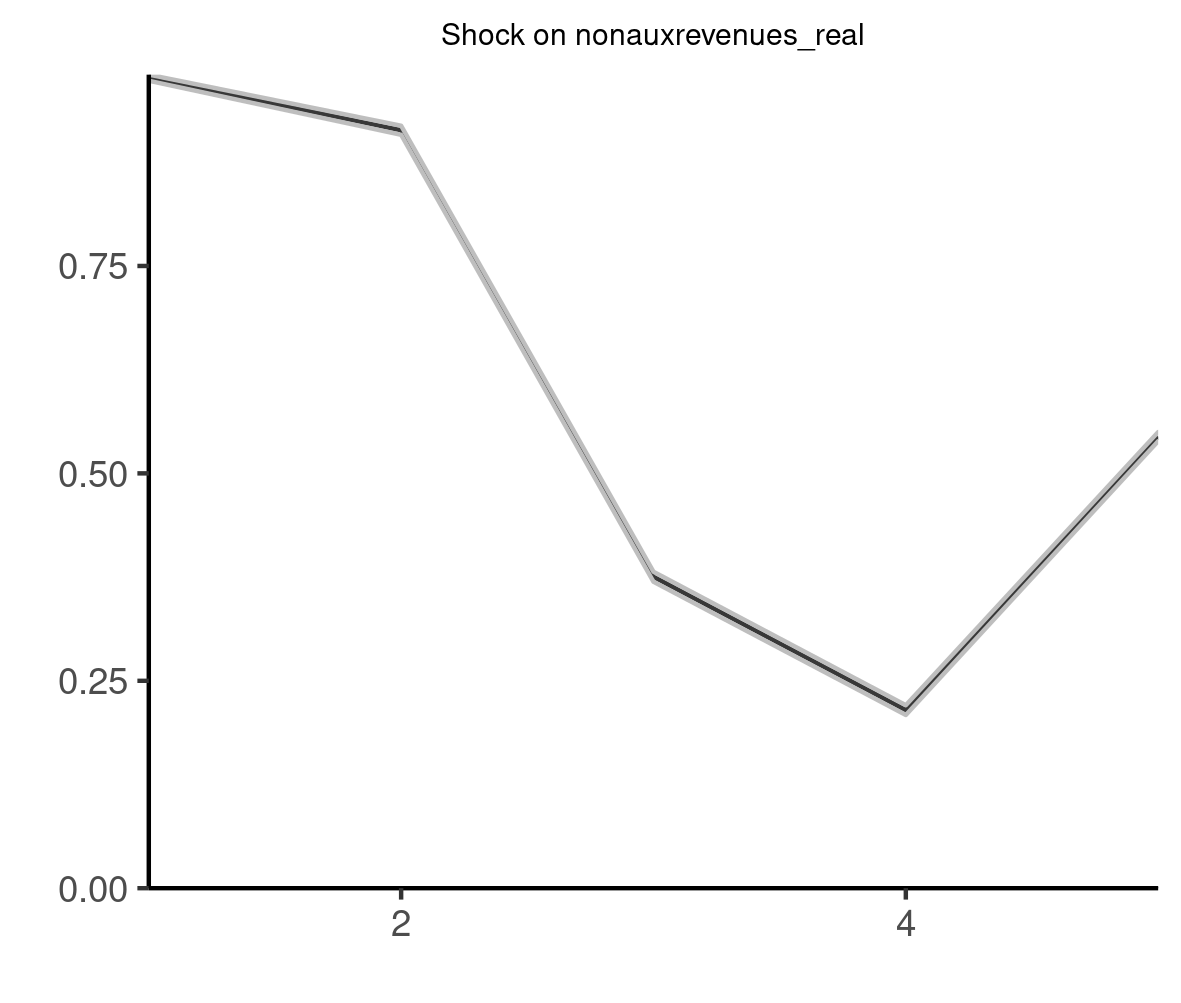
\includegraphics[width=0.6\textwidth]{figures/firststage-illinois-lp-rolling.png}
    \label{fig:firststage-illinois-lp}
\end{figure}


\subsection{Additional Results, University-Level}

\autoref{tab:facultysalaries-shock-reg} presents OLS and IV estimates where the outcome is (log) mean salary for professors employed at the university, separated by position.
Similarly, \autoref{fig:all-salaries-lp} shows the staying-power via projection methods.
The outcome, mean salary is crude.

\begin{table}[H]
    \singlespacing
    \centering
    \caption{OLS and 2SLS Estimates for University Faculty-Tenure Composition.}
    \makebox[\textwidth][c]{
\begin{tabular}{@{\extracolsep{5pt}}lcccccccc} 
\\[-1.8ex]\hline 
\hline \\[-1.8ex] 
 & \multicolumn{8}{c}{Dependent Variable: Employment Count by Tenure Group} \\ 
\cline{2-9} 
\\[-1.8ex] & \multicolumn{2}{c}{Non-tenure} & \multicolumn{2}{c}{Tenure-Track} & \multicolumn{2}{c}{Tenured} & \multicolumn{2}{c}{All} \\ 
 & OLS & 2SLS & OLS & 2SLS & OLS & 2SLS & OLS & 2SLS \\ 
\\[-1.8ex] & (1) & (2) & (3) & (4) & (5) & (6) & (7) & (8)\\ 
\hline \\[-1.8ex] 
 State Funding & $-$0.0004 & 1.499 & 0.048 & 1.926 & 0.051 & 0.267 & 0.037 & 0.893 \\ 
  & (0.016) & (10.764) & (0.051) & (8.050) & (0.029) & (1.104) & (0.023) & (4.610) \\ 
 \hline \\[-1.8ex] 
Observations & 4,825 & 4,825 & 5,094 & 5,094 & 5,130 & 5,130 & 5,181 & 5,181 \\ 
R$^{2}$ & 0.849 & 0.588 & 0.777 & $-$0.413 & 0.898 & 0.872 & 0.932 & 0.426 \\ 
\hline 
\hline \\[-1.8ex] 
\end{tabular} 
}
    \begin{flushleft}
        \footnotesize
        \textbf{Note}: Standard errors are clustered at the university-year level.
    \end{flushleft}
    \label{tab:tenurecount-shock-reg-fte}
\end{table}

\begin{table}[H]
    \singlespacing
    \centering
    \caption{OLS and 2SLS Estimates for University Faculty Salaries.}
    \makebox[\textwidth][c]{
\begin{tabular}{@{\extracolsep{5pt}}lcccccccc} 
\\[-1.8ex]\hline 
\hline \\[-1.8ex] 
 & \multicolumn{8}{c}{Dependent Variable: Mean Salary by Professor Group} \\ 
\cline{2-9} 
\\[-1.8ex] & \multicolumn{2}{c}{Lecturer} & \multicolumn{2}{c}{Assistant} & \multicolumn{2}{c}{Full} & \multicolumn{2}{c}{All} \\ 
 & OLS & 2SLS & OLS & 2SLS & OLS & 2SLS & OLS & 2SLS \\ 
\\[-1.8ex] & (1) & (2) & (3) & (4) & (5) & (6) & (7) & (8)\\ 
\hline \\[-1.8ex] 
 Appropriations Shock & 0.039 & 0.135 & 0.032 & 0.078 & 0.042 & 0.135 & $-$0.031 & 0.089 \\ 
  & (0.013) & (0.068) & (0.017) & (0.063) & (0.018) & (0.081) & (0.036) & (0.142) \\ 
  Tuition Revenue & 0.010 & $-$0.026 & 0.048 & 0.030 & 0.043 & 0.007 & 0.049 & 0.002 \\ 
  & (0.015) & (0.027) & (0.013) & (0.026) & (0.016) & (0.032) & (0.031) & (0.057) \\ 
 \hline \\[-1.8ex] 
Observations & 16,260 & 16,260 & 17,212 & 17,212 & 17,317 & 17,317 & 17,397 & 17,397 \\ 
R$^{2}$ & 0.682 & 0.678 & 0.823 & 0.822 & 0.855 & 0.851 & 0.412 & 0.411 \\ 
\hline 
\hline \\[-1.8ex] 
\end{tabular} 
}
    \begin{flushleft}
        \footnotesize
        \textbf{Note}: Standard errors are clustered at the state-year level.
    \end{flushleft}
    \label{tab:facultysalaries-shock-reg}
\end{table}

\begin{figure}[H]
    \centering
    \singlespacing
    \caption{Local Projection Estimates for Professor Salary, Mean within Each University.}
    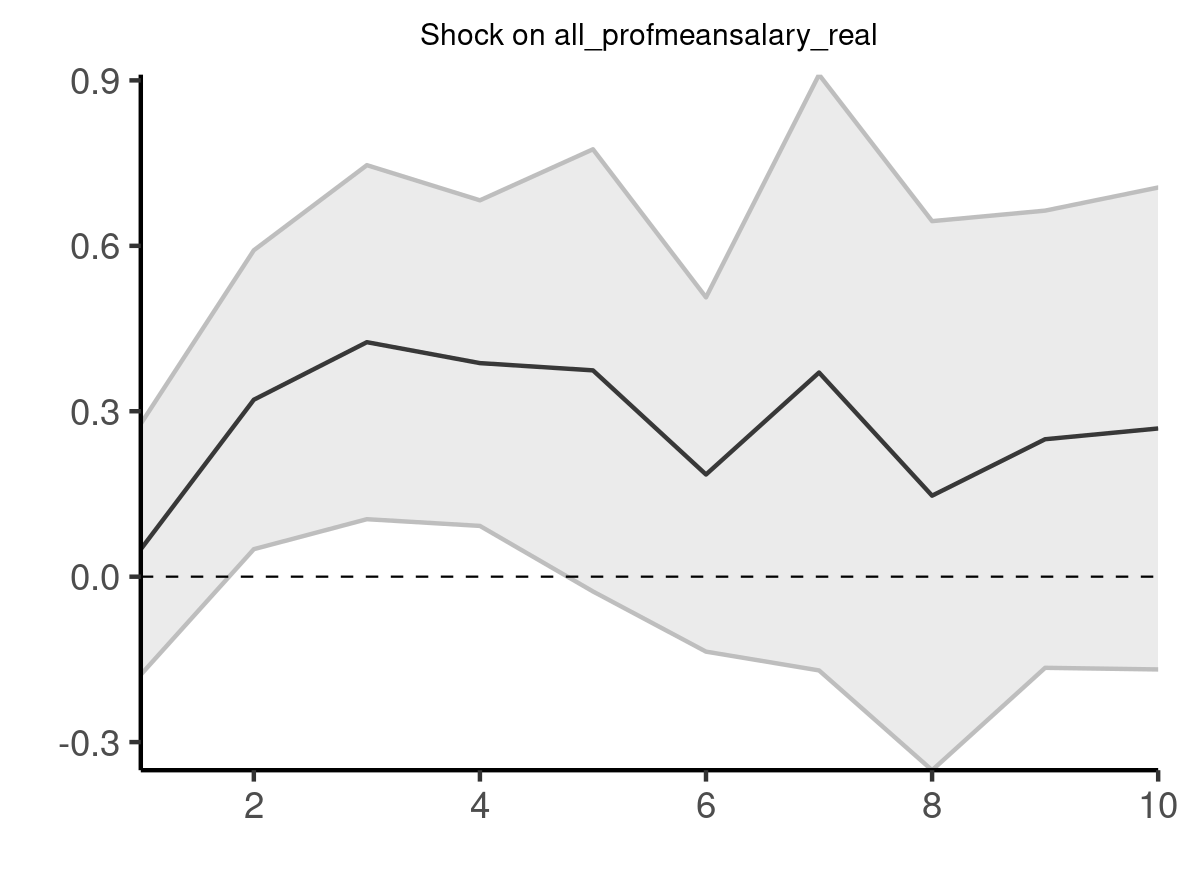
\includegraphics[width=0.6\textwidth]{figures/all-salaries-lp.png}
    \label{fig:all-salaries-lp}
\end{figure}


\subsection{Additional Results, Individual-Professor Level}

\begin{table}[H]
    \singlespacing
    \centering
    \caption{2SLS Estimates for Faculty Salaries at Illinois Universities.}
    \makebox[\textwidth][c]{
\begin{tabular}{@{\extracolsep{5pt}}lccccc} 
\\[-1.8ex]\hline 
\hline \\[-1.8ex] 
 & \multicolumn{5}{c}{Dependent Variable: Salaries by Professor Group} \\ 
\cline{2-6} 
 & Lecturer & Assistant & Full & Admin & All \\ 
\\[-1.8ex] & (1) & (2) & (3) & (4) & (5)\\ 
\hline \\[-1.8ex] 
 Non-inst. Revenues & $-$0.306 & $-$0.216 & $-$0.069 & $-$0.117 & $-$0.222 \\ 
  & (0.139) & (0.105) & (0.030) & (0.097) & (0.133) \\ 
  Tuition Revenue & 0.769 & $-$0.416 & 0.005 & 0.468 & 0.740 \\ 
  & (0.465) & (0.310) & (0.106) & (0.246) & (0.309) \\ 
 \hline \\[-1.8ex] 
Observations & 49,637 & 39,051 & 68,243 & 28,639 & 185,570 \\ 
R$^{2}$ & 0.185 & 0.064 & 0.078 & 0.130 & 0.140 \\ 
\hline 
\hline \\[-1.8ex] 
\end{tabular} 
}
    \begin{flushleft}
        \footnotesize
        \textbf{Note}: Standard errors are clustered at the institution-year level.
    \end{flushleft}
    \label{tab:facultysalaries-shock-illinois}
\end{table}

\begin{table}[H]
    \singlespacing
    \centering
    \caption{2SLS Estimates for Faculty Promotion Rate at Illinois Universities, using Rolling Instrument.}
    \makebox[\textwidth][c]{
\begin{tabular}{@{\extracolsep{5pt}}lcccc} 
\\[-1.8ex]\hline 
\hline \\[-1.8ex] 
 & \multicolumn{4}{c}{Dependent Variable: Promotion Rate by Professor Group} \\ 
\cline{2-5} 
 & Lecturer & Assistant & Associate & All \\ 
\\[-1.8ex] & (1) & (2) & (3) & (4)\\ 
\hline \\[-1.8ex] 
 Non-inst. Revenues & 0.014 & 0.035 & 0.029 & 0.014 \\ 
  & (0.007) & (0.019) & (0.062) & (0.009) \\ 
 \hline \\[-1.8ex] 
Observations & 16,346 & 17,094 & 4,377 & 42,396 \\ 
R$^{2}$ & 0.007 & 0.024 & 0.029 & 0.009 \\ 
\hline 
\hline \\[-1.8ex] 
\end{tabular} 
}
    \begin{flushleft}
        \footnotesize
        \textbf{Note}: Standard errors are clustered at the institution and first year of employment level.
    \end{flushleft}
    \label{tab:promotion-shock-illinois-rolling}
\end{table}

\begin{table}[H]
    \singlespacing
    \centering
    \caption{2SLS Estimates for Faculty Promotion Rate at Illinois Universities, using Base-Year Instrument.}
    \makebox[\textwidth][c]{
\begin{tabular}{@{\extracolsep{5pt}}lcccc} 
\\[-1.8ex]\hline 
\hline \\[-1.8ex] 
 & \multicolumn{4}{c}{Dependent Variable: Promotion Rate by Professor Group} \\ 
\cline{2-5} 
 & Lecturer & Assistant & Associate & All \\ 
\\[-1.8ex] & (1) & (2) & (3) & (4)\\ 
\hline \\[-1.8ex] 
 Non-inst. Revenues & 0.051 & 0.063 & $-$0.002 & 0.010 \\ 
  & (0.028) & (0.031) & (0.036) & (0.013) \\ 
  Tuition Revenue & $-$0.086 & $-$0.180 & $-$0.231 & 0.008 \\ 
  & (0.040) & (0.061) & (0.082) & (0.024) \\ 
 \hline \\[-1.8ex] 
Observations & 36,097 & 39,527 & 35,978 & 135,221 \\ 
R$^{2}$ & 0.014 & 0.019 & 0.027 & 0.004 \\ 
\hline 
\hline \\[-1.8ex] 
\end{tabular} 
}
    \begin{flushleft}
        \footnotesize
        \textbf{Note}: Standard errors are clustered at the institution and first year of employment level.
    \end{flushleft}
    \label{tab:promotion-shock-illinois}
\end{table}

\begin{figure}[H]
    \centering
    \singlespacing
    \caption{Local Projection Estimates for Promotion Rate at Illinois Universities.}
    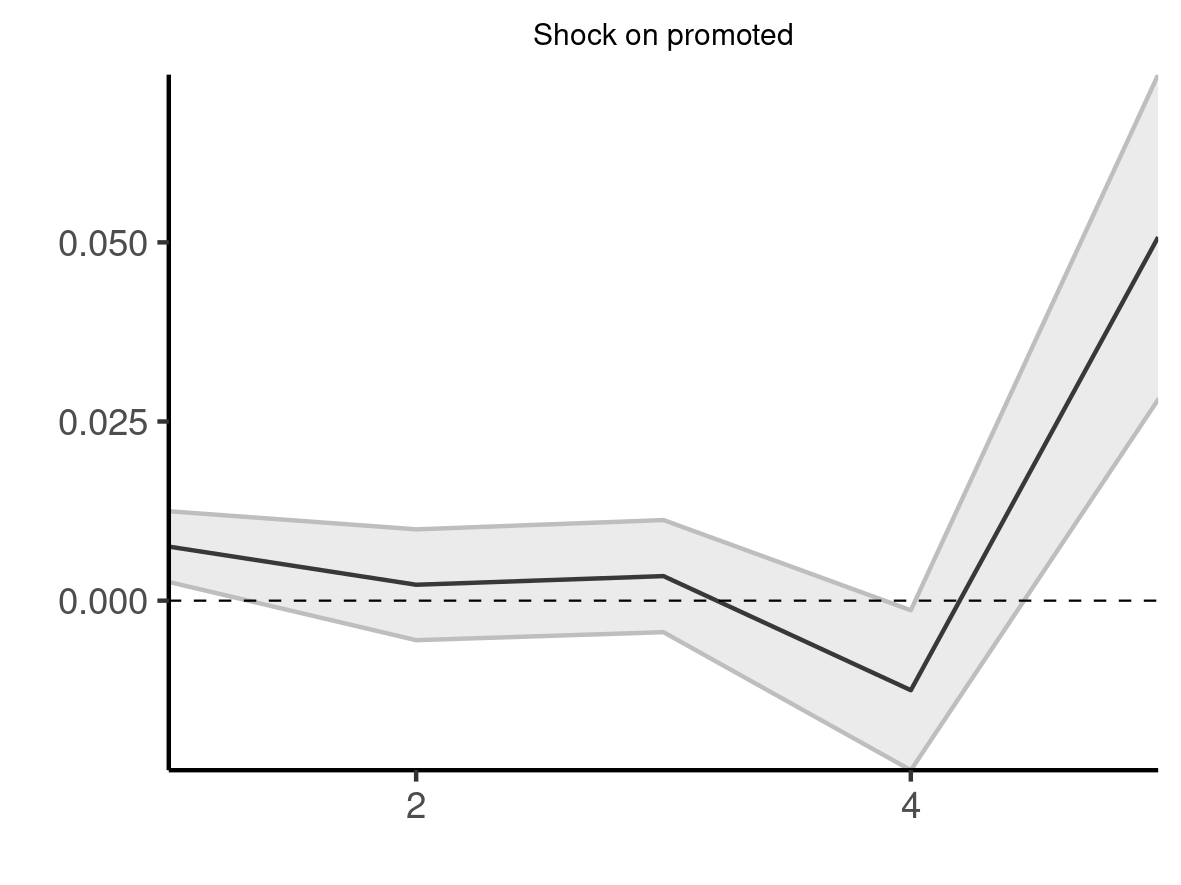
\includegraphics[width=0.6\textwidth]{figures/promoted-illinois-lp-rolling.png}
    \label{fig:promoted-illinois-lp}
\end{figure}

\begin{table}[H]
    \singlespacing
    \centering
    \caption{2SLS Estimates for Faculty Exit Rate at Illinois Universities, using Rolling Instrument.}
    \makebox[\textwidth][c]{
\begin{tabular}{@{\extracolsep{5pt}}lccccc} 
\\[-1.8ex]\hline 
\hline \\[-1.8ex] 
 & \multicolumn{5}{c}{Dependent Variable: Exit rate by Professor Group} \\ 
\cline{2-6} 
 & Lecturer & Assistant & Full & Admin & All \\ 
\\[-1.8ex] & (1) & (2) & (3) & (4) & (5)\\ 
\hline \\[-1.8ex] 
 Non-inst. Revenues & $-$0.007 & 0.002 & $-$0.004 & $-$0.003 & $-$0.006 \\ 
  & (0.024) & (0.006) & (0.008) & (0.020) & (0.015) \\ 
 \hline \\[-1.8ex] 
Observations & 23,376 & 19,757 & 7,190 & 10,191 & 60,514 \\ 
R$^{2}$ & 0.013 & 0.006 & 0.014 & 0.068 & 0.016 \\ 
\hline 
\hline \\[-1.8ex] 
\end{tabular} 
}
    \begin{flushleft}
        \footnotesize
        \textbf{Note}: Standard errors are clustered at the institution and first year of employment level.
    \end{flushleft}
    \label{tab:facultyleaving-shock-illinois-rolling}
\end{table}

\begin{table}[H]
    \singlespacing
    \centering
    \caption{2SLS Estimates for Faculty Exit Rate at Illinois Universities, using Base-Year Instrument.}
    \makebox[\textwidth][c]{
\begin{tabular}{@{\extracolsep{5pt}}lccccc} 
\\[-1.8ex]\hline 
\hline \\[-1.8ex] 
 & \multicolumn{5}{c}{Dependent Variable: Exit rate by Professor Group} \\ 
\cline{2-6} 
 & Lecturer & Assistant & Full & Admin & All \\ 
\\[-1.8ex] & (1) & (2) & (3) & (4) & (5)\\ 
\hline \\[-1.8ex] 
 Non-inst. Revenues & $-$0.009 & 0.0001 & 0.001 & 0.018 & 0.004 \\ 
  & (0.015) & (0.003) & (0.003) & (0.020) & (0.009) \\ 
 \hline \\[-1.8ex] 
Observations & 45,734 & 35,882 & 62,499 & 26,337 & 170,452 \\ 
R$^{2}$ & 0.030 & 0.005 & 0.003 & 0.026 & 0.016 \\ 
\hline 
\hline \\[-1.8ex] 
\end{tabular} 
}
    \begin{flushleft}
        \footnotesize
        \textbf{Note}: Standard errors are clustered at the institution and first year of employment level.
    \end{flushleft}
    \label{tab:facultyleaving-shock-illinois}
\end{table}